\chapter{The Project}

\section{Human Robot Interaction Package for ROS}

%% USE A DESCRIPRIVE TITLE! (ie. Robot Brain Implementation)
%% See your choises in birds eye perspective. how you can discuss what youve done.


%% What was made, why is it good. document all choices. The rule is that a different scientist with the same resources should be able to get the same results based on your description. Dont write about the methods in general, but exactly what youre doing. discuss your own approach. Show that youre aware there are other alternatives to what you did, and what advantages a different method may have. Did you have any influence over how things were solved. what is strengths and weaknesses about your work. what would you do different if you were to do it again? be open about weaknesses, but defend your choices. Refer to other researchers who has done the same. 

A multipurpose package for tracking information about humans was made. The package features both detection of 2D joints as well as a method of manually fitting a whole 3D skeleton to the observed points.

\section{Human Pose Estimation}

The robot we're developing needs to be able to robustly detect humans, so information about their state can be gathered and analyzed. To accomplish this task, we propose a system that uses RGB-D data in combination with IR images to estimate the 3D pose of humans. In addition we propose a manual algorithm for estimation of occluded parts that can not be directly observed. 

A lot of work has already been done on human pose estimation, however this approach focuses on creating a manual method for constraining the 3D skeleton and estimating the 3D pose of the observed person. We rely on 2D detection of joints for each person by the OpenPose software. 

\begin{figure}
  \centering
  \begin{floatrow}
    \ffigbox[.3\textwidth]{
      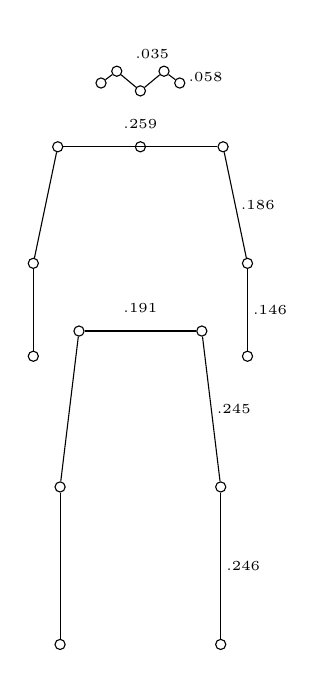
\begin{tikzpicture}[
          every node/.style={draw,circle,minimum size=.06cm, inner sep=1.3pt}
        ]
        \tiny
        %% \draw[help lines, step=5mm, gray!20] (-4,-4) grid (3,4);
        
        \node (nose) at (0,3.25) {};
        \node (neck) at (0,2.54) {};
        
        \node (reye) at (-.3,3.5) {};
        \node (leye) at (.3,3.5) {};

        \node (rear) at (-.5,3.35) {};
        \node (lear) at (.5,3.35) {};

        \node (rshoulder) at (-1.05,2.54) {};
        \node (lshoulder) at (1.05,2.54) {};
        
        \node (relbow) at (-1.36,1.06) {};
        \node (lelbow) at (1.36,1.06) {};

        \node (rwrist) at (-1.36,-.12) {};
        \node (lwrist) at (1.36,-.12) {};

        \node (rhip) at (-.78,.2) {};
        \node (lhip) at (.78,.2) {};

        \node (rknee) at (-1.02,-1.78) {};
        \node (lknee) at (1.02,-1.78) {};

        \node (rankle) at (-1.02,-3.78) {};
        \node (lankle) at (1.02,-3.78) {};

        %% \draw[blue] (0,0) circle [radius=.06cm];

        \draw (reye) -- (nose); \draw (leye) -- node[above, draw=none, inner sep=2.5pt] {.035} ++(nose);
        \draw (reye) -- (rear); \draw (leye) -- node[right, draw=none, inner sep=4.3pt] {.058} ++(lear);

        %% \draw (rear) -- node[below right, draw=none, xshift=5pt] {.105} ++(lear);
        
        \draw (lshoulder) -- node[above, draw=none] {.259} ++(rshoulder);

        \draw (rshoulder) -- (relbow); \draw (lshoulder) -- node[right, draw=none] {.186} ++(lelbow);
        \draw (rwrist) -- (relbow); \draw (lwrist) -- node[right, draw=none] {.146} ++(lelbow);

        \draw (rhip) -- (rknee); \draw (lhip) -- node[right, draw=none] {.245} ++(lknee);
        \draw (rknee) -- (rankle); \draw (lknee) -- node[right, draw=none] {.246} ++(lankle);

        \draw (rhip) -- node[above, draw=none] {.191} ++(lhip);
      \end{tikzpicture}
    }
    {
      \label{fig:constrained_lengths}
      \caption[Constrained Lenghts]{Constrained limb connections.}
    }
    %% \end{figure}
    %% \begin{table}
    \capbtabbox{
      \begin{tabular}[H]{|r l|l|c|}
        \hline
        ID & Limb & Model & Pair \\ %%& $\pm\bm{t}$ \\
        \hline
        0 & Left arm & .186 & 5 -- 6 \\ %% & .05 \\
        1 & Left forearm & .146 & 6 -- 7 \\ %%&.05 \\
        2 & Right arm & .186 & 2 -- 3 \\ %%& .05\\
        3 & Right forearm & .146 & 3 -- 4 \\ %%& .05\\
        4 & Hip & .191 & 8 -- 11 \\ %%& .06\\
        5 & Left thigh & .245 & 11 -- 12 \\ %%& .07 \\
        6 & Left leg & .246 & 12 -- 13 \\ %%& .07 \\
        7 & Right thigh & .245 & 8 -- 9 \\ %%& .07 \\
        8 & Right leg & .246 & 9 -- 10 \\ \hline %%& .07 \\ \hline
      %%   $\lvert Right shoulder - Right elbow\rvert = \lvert Left shoulder - Left elbow \rvert$
      %%   \hline
      \end{tabular}
    }{
      \label{tab:constrain_rules}
      \caption[Anthropometry constrain rules]{Constrain rules for correct anthropometry. (Note that the anthropometry for the head and shoulders are not yet implemented.)}
    }
  \end{floatrow}
\end{figure}

\subsection{Formulas for constraining}

For a fixed point $a$ we want to move a point $b$ so the Euclidean distance between them is equal to $L$. A few different methods was developed to accomplish this, based on the reliability of the different keypoints.

\subsubsection{Keypoint projection}
If both $\vec{a}$ and $\vec{b}$ are well-observed points and the initial distance between the point $\vec{a}$ and the line from the camera center through $\vec{b}$ are less than $L$, we use the following formula to calculate the new position of $\vec{b}$.
We get the length, $x$ of the vector to the new position of $\vec{b}$ by using equation~\ref{eq:pushvector}. The constrained point is then simply defined as $x|\vec{b}|$.
\begin{equation}
  x = \max\left(\frac{2(\vec{a} \boldsymbol{\cdot} \vec{b}) \pm \sqrt{4(\vec{a} \boldsymbol{\cdot} \vec{b})^{2} - 4 ||\vec{b}||^{2} (||\vec{a}||^{2} - L^{2})}}{2 (||\vec{a}||^{2} - L^{2})}\right)
  \label{eq:pushvector}
\end{equation}
However, if the minimum distance between $\vec{b}$ and the line is more than $L$, we define the point as the point $L$ away from point $\vec{a}$ on the line through the coordinates of $\vec{a}$ perpendicular to the line along $\vec{b}$. The point is then defined by equation~\ref{eq:perpendicular}.
\begin{equation}
  \vec{p} = \vec{a} + L\left|\vec{a} - \frac{\vec{a}\boldsymbol{\cdot}\vec{b}}{\vec{b}\boldsymbol{\cdot}\vec{b}} \boldsymbol{\cdot} \vec{b}\right|
  \label{eq:perpendicular}
\end{equation}

\subsubsection{Keypoint interpolation}
This method could be used both to create one additional keypoint, or to determine the location of an obstructed keypoint. We assume we again have two well observed keypoints $a$ and $c$. We wish to find the location of keypoint $b$.
To interpolate, we imagine two spheres around point $a$ and $c$ with radiuses $r_a, r_c$. The interpolated point must be on the intersecting circle between the two spheres. The distance from point $a$ to the plane of that circle is defined as $x = \frac{d^2 - r_c^2 + r_a^2}{2d}$ where $d$ is the Euclidean distance $||a - c||$. The radius of the circle is defined as $h = \frac{1}{d}\sqrt{(-d+r_c-r_a)(-d-r_c-r_a)(-d+r_c+r_a)(d+r_c+r_a)}$. The keypoint $b$ is then defined as the keypoint furthest away from the camera on this circle. In later versions this could be constrained by the angle between the previous limb and this one.

\subsection{Skeleton fitting}

We wish to fit a constrained skeleton to the observed points in 3D space. Our skeleton is defined as three separate graphs with constrained edges.
The keypoints defining the nodes of the graphs (joints) are detected by the OpenPose network, and sorted based on the confidence of detection. For each graph a subset of $n$ keypoints are picked as seeds, and constrained graphs are generated:\\
Scale (and thus limb length) is calculated based on the confidence of the keypoints using the weighted sum in equation~\ref{eq:scale} where $L$ is the set of Euclidean lengths in each graph and $S$ is the scores of those lengths. $S$ is calculated by the Gaussian function of the confidence of the scores $c_a$ and $c_b$ with $\sigma = 0.33$ as described in equation~\ref{eq:limb_score}.
\begin{equation}
  S = \frac{\sum_{i=0}^{N}L(i) \cdot s(i)}{\sum_{i=0}^{N}s(i)}
  \label{eq:scale}
\end{equation}
\begin{equation}
  s = \frac{1}{\sqrt{\sigma\pi}}e^{-\frac{1}{\sigma}(c_a-1)^2 + (c_b -1)^2}
  \label{eq:limb_score}
\end{equation}
    {\color{red} Alternative notation for equation~\ref{eq:limb_score} because of possible cumbersome notation in $e$ expression.
\[
s = \frac{1}{\sqrt{\sigma\pi}}{\exp}\left(-\frac{1}{\sigma}(c_a-1)^2 + (c_b -1)^2\right)
\]}
We then recursively constrain all points based on a seed point from the sorted keypoints. If no keypoints with confidence over a certain threshold $t$ are detected, the graph is not placed.
The constrained graph is moved to the center of the detected keypoint, again weighted by $S$, and we are finished constraining the graph.

The skeleton is defined as the subset of graphs best matching their respective keypoints where scale is similar.
